\documentclass[12pt]{article}
\usepackage{graphicx}
\usepackage{amsmath}

\title{Multi-Layer Perceptron (MLP) for Wine Quality Classification}
\author{Your Name}
\date{\today}

\begin{document}

\maketitle

\section{Introduction}
This project focuses on building a basic Multi-Layer Perceptron (MLP) from scratch using NumPy to classify wine quality based on physicochemical properties. The dataset used for this classification contains characteristics such as acidity, pH, and alcohol content, as well as the quality rating of the wines. The project includes both theoretical and practical tasks, including data preprocessing, model implementation, and evaluation using various learning rates.

\section{Dataset Description}
The dataset used in this project is the Wine Quality Dataset, which includes both red and white wines. For the purpose of this assignment, we focus on the red wine dataset. The dataset contains the following features:

\begin{itemize}
    \item Fixed acidity
    \item Volatile acidity
    \item Citric acid
    \item Residual sugar
    \item Chlorides
    \item Free sulfur dioxide
    \item Total sulfur dioxide
    \item Density
    \item pH
    \item Sulphates
    \item Alcohol
    \item Quality (score between 0 and 10)
\end{itemize}

\section{Methodology}
\subsection{Data Preprocessing}
The red wine dataset was loaded using NumPy and preprocessed by normalizing and standardizing the features. The dataset was then split into training and testing sets with an 80\% to 20\% ratio, respectively.

\subsection{Model Architecture}
We implemented a basic MLP from scratch, starting with a simple architecture containing one hidden layer. The number of input nodes corresponds to the features of the wine, while the output node corresponds to the quality rating.

\subsection{Training Process}
The model was trained using the backpropagation algorithm, with a learning rate range from $1 \times 10^{-8}$ to 10. We evaluated the loss reduction over training iterations for each learning rate.

\section{Results}
\subsection{Loss Reduction with Different Learning Rates}
The following plots show the loss reduction across 10,000 iterations for different learning rates:

\begin{figure}[h!]
    \centering
    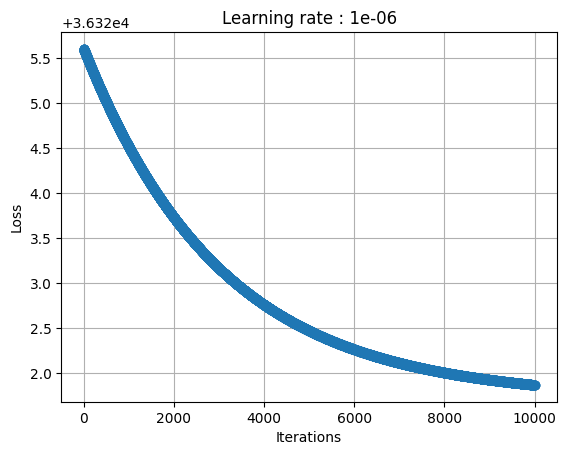
\includegraphics[width=0.7\textwidth]{plot_28.png}
    \caption{Learning rate: 1e-06}
    \label{fig:lr1e-06}
\end{figure}

\begin{figure}[h!]
    \centering
    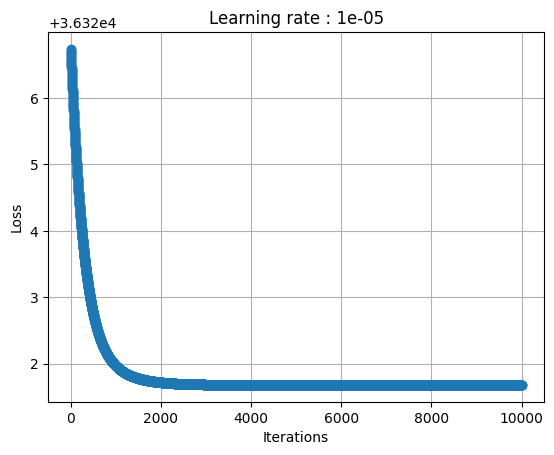
\includegraphics[width=0.7\textwidth]{plot_29.png}
    \caption{Learning rate: 1e-05}
    \label{fig:lr1e-05}
\end{figure}

\begin{figure}[h!]
    \centering
    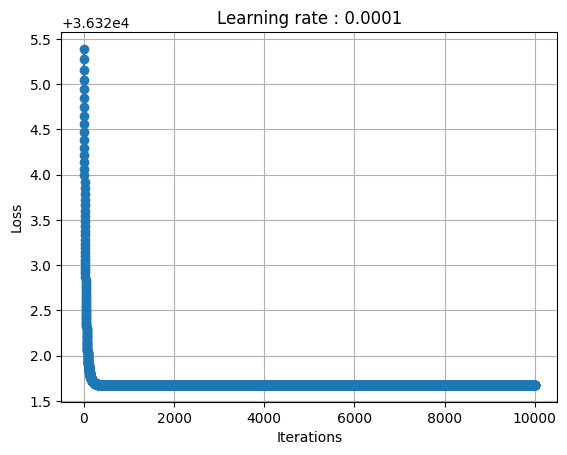
\includegraphics[width=0.7\textwidth]{plot_30.png}
    \caption{Learning rate: 0.0001}
    \label{fig:lr0.0001}
\end{figure}

\begin{figure}[h!]
    \centering
    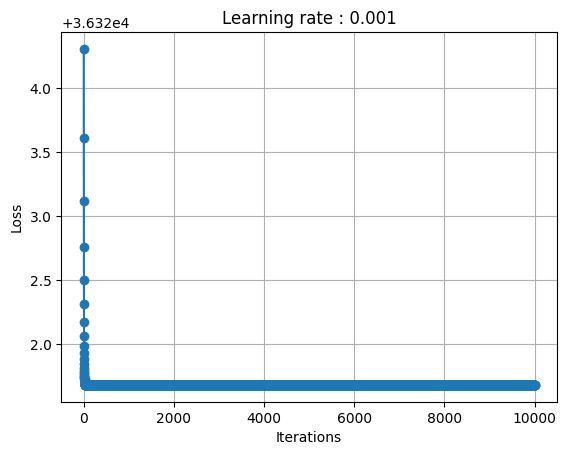
\includegraphics[width=0.7\textwidth]{plot_31.png}
    \caption{Learning rate: 0.001}
    \label{fig:lr0.001}
\end{figure}

\begin{figure}[h!]
    \centering
    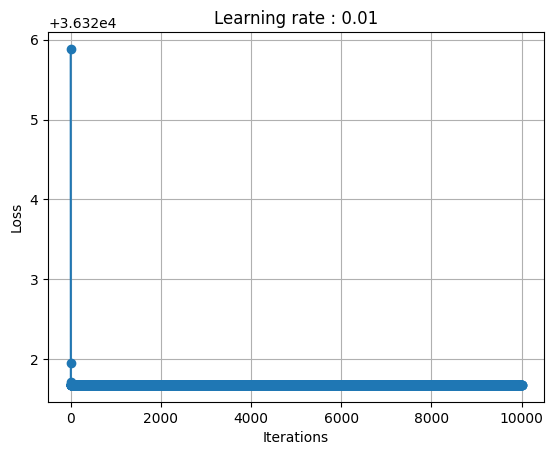
\includegraphics[width=0.7\textwidth]{plot_32.png}
    \caption{Learning rate: 0.01}
    \label{fig:lr0.01}
\end{figure}

\begin{figure}[h!]
    \centering
    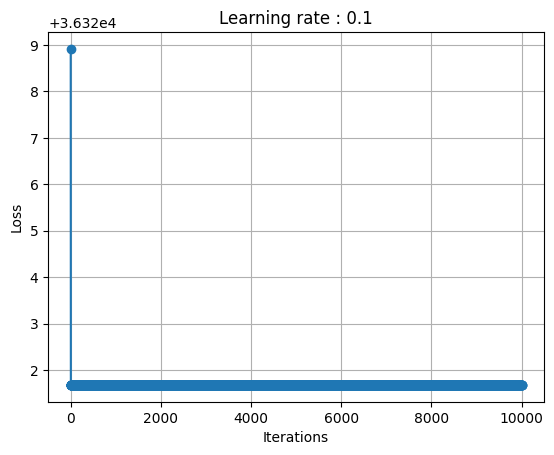
\includegraphics[width=0.7\textwidth]{plot_33.png}
    \caption{Learning rate: 0.1}
    \label{fig:lr0.1}
\end{figure}

\subsection{Model Performance}
The model's performance was evaluated based on several metrics, including accuracy, precision, recall, and F1-score. These metrics helped assess how well the model generalizes to unseen data.

\section{Analysis}
The results from training with different learning rates demonstrate how the learning rate impacts convergence. Higher learning rates tend to cause unstable training, while lower rates lead to slower convergence. By observing the loss curves, we can conclude the optimal learning rate for this specific task.

\section{Conclusion}
In this project, we successfully implemented an MLP to classify wine quality using the red wine dataset. We observed the effects of different learning rates on model performance, and the results highlighted the importance of choosing the appropriate learning rate for optimal convergence.

\section{References}
\begin{itemize}
    \item Wine Quality Dataset: \url{https://www.kaggle.com/datasets/yasserh/wine-quality-dataset}
\end{itemize}

\end{document}
